\documentclass[12pt]{article}
\usepackage{amsmath}
\setlength{\jot}{2ex}
\usepackage{mathrsfs}
\usepackage{steinmetz}
\usepackage{graphicx}
\usepackage{wrapfig}
\usepackage{booktabs}
\usepackage[letterpaper, margin=1in]{geometry}
\usepackage{fancyhdr}
\pagestyle{fancy}
\fancyhead[R]{Steady-State Power}
\fancyfoot[C]{\thepage}
\renewcommand{\headrulewidth}{1pt}
\renewcommand{\footrulewidth}{1pt}
\usepackage [autostyle, english = american]{csquotes}
\MakeOuterQuote{"}
\renewcommand{\baselinestretch}{1.0}
\newcommand{\objects}[2]{%
  \leavevmode\vbox{\hbox{#1}\nointerlineskip\hbox{#2}}%
}
\begin{document}
    \section*{Instantaneous Power}
    In general, power is equal to $vi$, where $v$ is the voltage and $i$ is the
    current. In this case, since the voltage and the current are given by
    sinusoidal functions,
    \begin{gather*}
        v = V_{m} \cos (\omega t + \theta_{v}), \\
        i = I_{m} \cos (\omega t + \theta_{i})
    \end{gather*}
    power can be represented as,
    \[
        p = V_{m}I_{m} \cos (\omega t + \theta_{v}) \cos (\omega t + \theta_{i})
    .\]
    Now instead of dealing with both the phase angles for the current and the
    voltage, the expressions can be written as,
    \begin{gather*}
        v = V_{m} \cos (\omega t + \theta_{v} - \theta_{i}), \\
        i = I_{m} \cos (\omega t), \\
        p = V_{m}I_{m} \cos (\omega t + \theta_{v} - \theta_{i}) \cos (\omega t)
    .\end{gather*}
    Using the trigonometric identity,
    \[
        \cos (\alpha) \cos (\beta) = \frac{1}{2} (\cos (\alpha - \beta) + \cos
        (\alpha + \beta))
    ,\]
    where $\alpha = \omega t + \theta_{v} - \theta_{i}$ and $\beta = \omega t$,
    \[
        p = \frac{V_{m} I_{m}}{2} \cos (\theta_{v} - \theta_{i}) + \frac{V_{m}
        I_{m}}{2} \cos (2 \omega t + \theta_{v} - \theta_{i})
    .\]
    Using the identity,
    \[
        \cos (\alpha + \beta) = \cos (\alpha) \cos (\beta) - \sin (\alpha) \sin
        (\beta)
    ,\]
    the expression can be expanded to be written as,
    \[
        \boxed{p = \frac{V_{m} I_{m}}{2} \cos (\theta_{v} - \theta_{i}) +
        \frac{V_{m} I_{m}}{2} \cos (\theta_{v} - \theta_{i}) \cos (2 \omega t) -
        \frac{V_{m} I_{m}}{2} \sin (\theta_{v} - \theta_{i}) \sin (2 \omega t).}
    \]
    \section*{Average and Reactive Power}
    The expression for instantaneous power seems daunting however, it can be
    broken into parts where each part is significant in its own regard,
    \[
        p = P + P \cos (2 \omega t) - Q \sin (2 \omega t)
    .\]
    \\ \textbf{Average (Real) Power:}
    \[
        P = \frac{V_{m} I_{m}}{2} \cos (\theta_{v} - \theta_{i})
    \]
    \\ \textbf{Reactive Power:}
    \[
        Q = \frac{V_{m} I_{m}}{2} \sin (\theta_{v} - \theta_{i})
    \]
    \newpage
    \par Here, $P$ gives the average power while $Q$ gives the reactive power.
    The average power is referred to as the "real" power since it is power that
    is transformed from electric to non-electric energy within the circuit.
    \subsubsection*{Power for Purely Resistive Networks}
    \[
        p = P + P \cos (2 \omega t)
    \]
    \par For a purely resistive circuit the phases of the current and the
    voltage are equal, $\theta_{v} = \theta_{i}$, and with that the expression
    simplifies to the one above. Power cannot be extracted from a purely
    resistive network since resistors by nature dissipate energy in the form of
    heat.
    \subsubsection*{Power for Purely Inductive Networks}
    \[
        p = -Q \sin (2 \omega t)
    \]
    \par For a circuit containing only inductors the current lags the voltage by
    $90^{\circ}$ meaning, $\theta_{v} - \theta_{i} = 90^{\circ}$. With that, the
    expression simplifies to the one above as the cosine terms will be equal to
    zero.
    \par In a purely inductive circuit, the average power is zero as no energy
    is transformed from electric to non-electric, rather, the energy is
    continually transferred between the source that is driving the circuit and
    the coils of the inductors.
    \par The power in a purely inductive circuit is said to be reactive since
    the inductor itself is a reactive element in that, its impedance is
    completely reactive.
    \par The value of Average Power is given in \textit{watts}, W, while
    Reactive power is given in \textit{volt-ampere reactive}, VAR. This is due
    to the fact that both measurements of power are dimensionally identical.
    \subsubsection*{Power for Purely Capacitive Networks}
    \[
        p = -Q \sin (2 \omega t)
    \]
    \par With capacitors, the current leads the voltage by $90^{\circ}$ meaning
    $\theta_{v} - \theta_{i} = -90^{\circ}$. This leads once again to the
    expression for the Real part of the instantaneous power to equal zero,
    leaving purely the reactive power.
    \section*{The Power and Reactive Factors}
    \begin{gather*}
        \text{pf} = \cos (\theta_{v} - \theta_{i}), \\
        \text{rf} = \sin (\theta_{v} - \theta_{i})
    \end{gather*}
    \par The angle $\theta_{v} - \theta_{i}$ is used in both calculations of the
    average and reactive powers and for this reason, it is referred to as the
    power factor angle. The cosine of this angle in called the \textit{power
    factor} and the sine of the angle is known as the \textit{reactive factor}.
    \par Despite having the value of the power factor, the power factor angle
    cannot be determined since $\cos (\theta_{v} - \theta_{i}) = \cos (-
    (\theta_{v} - \theta_{i}))$. To completely describe the angle therefore, the
    phrases \textbf{lagging} and \textbf{leading} are used when describing the
    current and voltage in the circuit. A lagging power factor means that the
    current lags the voltage, the load is inductive. A leading power factor
    means that the current is leading the voltage, the load is capacitive.
    \section*{The rms Values in Power Calculations}
    \begin{gather*}
        P = \frac{V_{rms}^2}{R}, \\
        P = I_{rms}^2 R
    \end{gather*}
    \par The rms value is also referred to as the effective value of the
    sinusoidal voltage or current. Given an equivalent resistive load, $R$, and
    an equivalent time period for the voltage and current, the rms value of a
    sinusoidal source delivers the same energy to $R$ as does a $dc$ source of
    the same value.
    \section*{Complex Power}
    \[
        S = P + j Q
    \]
    \par Complex Power has the same units as average and reactive power. To
    distinguish it from the other two, the units given to it are
    \textit{volt-amps}, VA.
    \begin{table}[h]
        \centering
        \begin{tabular}{cc}
            \toprule
            Quantity & Units \\
            \midrule
            Average Power & watts \\
            Reactive Power & volt-amps reactive \\
            Complex Power & volt-amps \\
            \bottomrule
        \end{tabular}
    \end{table}
    \subsubsection*{The Power Triangle}
    \begin{figure}[h]
        \centering
        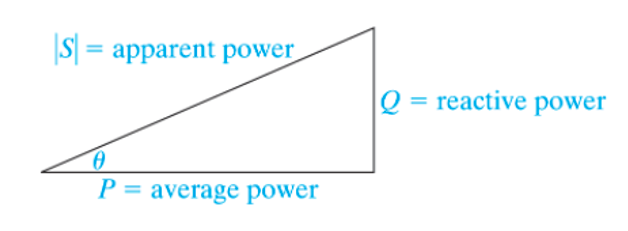
\includegraphics[width=0.45\textwidth]{Power Triangle.png}
    \end{figure}
    \noindent From the definitions of the different forms of power,
    \begin{gather*}
        \frac{Q}{P} = \frac{V_{m} I_{m} / 2\ \sin (\theta_{v} -
        \theta_{i})}{V_{m} I_{m} / 2\ \cos (\theta_{v} - \theta_{i})} \\
        \frac{Q}{P} = \tan (\theta_{v} - \theta_{i})
    \end{gather*}
    \textbf{Apparent Power}
    \[
        |S| = \sqrt{P^2+Q^2}
    \]
    \par From the triangle it can be seen that the angle $\theta$ is equal to
    the power factor angle, $\theta_{v} - \theta_{i}$. This relationship allows
    for the definition of apparent power, the magnitude of complex power.
    \par The apparent power, or volt-amp, requirement of a device designed to
    convert electrical energy to a non-electrical is more useful than the
    average power requirement. The apparent power represents the volt-amp
    capacity required to supply the average power used by the device. From the
    power triangle it can be seen that unless the power factor angle is
    $0^{\circ}$, the volt-amp capacity required is larger than the average power
    that will be used by the device.
    \section*{Power Calculations}
    \begin{align*}
        S &= \frac{V_{m} I_{m}}{2} \cos (\theta_{v} - \theta_{i}) + j \frac{V_{m}
          I_{m}}{2} \sin (\theta_{v} - \theta_{i}) \\
          &= \frac{V_{m} I_{m}}{2}\ [\cos (\theta_{v} - \theta_{i}) + j \sin
          (\theta_{v} - \theta_{i})] \\
          &= \frac{V_{m} I_{m}}{2}\ e^{j(\theta_{v} - \theta_{i})} = \frac{V_{m}
          I_{m}}{2}\ \phase{\theta_{v} - \theta_{i}}
    \end{align*}
    Using the rms values for both the current and the voltage,
    \begin{align*}
        S &= V_{rms} I_{rms} \phase{\theta_{v} - \theta_{i}} \\
          &= V_{rms} I_{rms} e^{j(\theta_{v} - \theta_{i})} \\
          &= V_{rms} e^{j \theta_{v}} I_{rms} e^{-j \theta_{i}}
    \end{align*}
    \subsubsection*{Complex Power, Alternate Form}
    \[
        S = \textbf{V}_{rms} \textbf{I}_{rms}^{*}
    \]
    \par Above is the formula to calculate the apparent power of a network given
    the rms values of the voltage and the current. It is defined as the phasor
    of the voltage multiplied by the complex conjugate of the current. If the
    values are not rms, the same derivation technique yields the formula,
    \[
        S = \frac{1}{2} \textbf{V} \textbf{I}^{*}
    .\]
    \par Using the same principles, other formulas can be defined for the
    apparent, reactive, and average power.
    \\ Since,
    \[
        \textbf{V}_{rms} = Z \textbf{I}_{rms}
    ,\]
    \begin{align*}
        S &= Z \textbf{I}_{rms} \textbf{I}_{rms}^{*} \\
          &= |\textbf{I}_{rms}|^2 Z \\
          &= |\textbf{I}_{rms}|^2 (R + jX) \\
          &= |\textbf{I}_{rms}|^2 R + j |\textbf{I}_{rms}|^2 X
    \end{align*}
    From this it can be seen that the values of $P$ and $Q$ can be given as,
    \[
        P = |\textbf{I}_{rms}|^{2} R = \frac{1}{2} \textbf{I}_{m}^2 R
    \]
    \[
        Q = |\textbf{I}_{rms}|^{2} X = \frac{1}{2} \textbf{I}_{m}^2 R
    \]
    Using the other general formula for power,
    \[
        S = \textbf{V}_{rms} \left( \frac{\textbf{V}_{rms}}{Z} \right)^{*} =
        \frac{|\textbf{V}_{rms}|^2}{Z^{*}}
    \]
    From this, as before, for a purely resistive element,
    \[
        P = \frac{|\textbf{V}_{rms}|^2}{R}
    ,\]
    and for a purely reactive element,
    \[
        Q = \frac{|\textbf{V}_{rms}|^2}{X}
    .\]
    \section*{Maximum Power Transfer}
    For a resistive circuit, it was found that in order for there to be a
    maximum amount of power transferred to the load, the Thevenin's resistance
    must be equal to the load resistance. For a circuit consisting of both
    resistive and reactive elements, the condition that must be met is for
    maximum power is,
    \[
        Z_{L} = Z_{TH}^{*}
    \]
    \subsubsection*{Maximum Average Power Absorbed}
    \[
        P_{max} = \frac{|V_{TH}|^2 R_{L}}{4 R_{L}^2} = \frac{1}{4}
        \frac{|V_{TH}|^2}{R_{L}}
    \]
\end{document}
